\documentclass[table]{article}
\usepackage{float}
\usepackage{lmodern}
\usepackage{amssymb,amsmath}
\usepackage{ifxetex,ifluatex}
\usepackage{fixltx2e} % provides \textsubscript
\ifnum 0\ifxetex 1\fi\ifluatex 1\fi=0 % if pdftex
  \usepackage[T1]{fontenc}
  \usepackage[utf8]{inputenc}
\else % if luatex or xelatex
  \ifxetex
    \usepackage{mathspec}
  \else
    \usepackage{fontspec}
  \fi
  \defaultfontfeatures{Ligatures=TeX,Scale=MatchLowercase}
\fi
% use upquote if available, for straight quotes in verbatim environments
\IfFileExists{upquote.sty}{\usepackage{upquote}}{}
% use microtype if available
\IfFileExists{microtype.sty}{%
\usepackage{microtype}
\UseMicrotypeSet[protrusion]{basicmath} % disable protrusion for tt fonts
}{}
\usepackage[margin=1in]{geometry}
\usepackage{hyperref}
\hypersetup{unicode=true,
            pdftitle={Report},
            pdfauthor={Nicolas Carmona, Niklas Tillenburg, Janek Teders},
            pdfborder={0 0 0},
            breaklinks=true}
\urlstyle{same}  % don't use monospace font for urls
\usepackage{color}
\usepackage{fancyvrb}
\newcommand{\VerbBar}{|}
\newcommand{\VERB}{\Verb[commandchars=\\\{\}]}
\DefineVerbatimEnvironment{Highlighting}{Verbatim}{commandchars=\\\{\}}
% Add ',fontsize=\small' for more characters per line
\usepackage{framed}
\definecolor{shadecolor}{RGB}{248,248,248}
\newenvironment{Shaded}{\begin{snugshade}}{\end{snugshade}}
\newcommand{\KeywordTok}[1]{\textcolor[rgb]{0.13,0.29,0.53}{\textbf{#1}}}
\newcommand{\DataTypeTok}[1]{\textcolor[rgb]{0.13,0.29,0.53}{#1}}
\newcommand{\DecValTok}[1]{\textcolor[rgb]{0.00,0.00,0.81}{#1}}
\newcommand{\BaseNTok}[1]{\textcolor[rgb]{0.00,0.00,0.81}{#1}}
\newcommand{\FloatTok}[1]{\textcolor[rgb]{0.00,0.00,0.81}{#1}}
\newcommand{\ConstantTok}[1]{\textcolor[rgb]{0.00,0.00,0.00}{#1}}
\newcommand{\CharTok}[1]{\textcolor[rgb]{0.31,0.60,0.02}{#1}}
\newcommand{\SpecialCharTok}[1]{\textcolor[rgb]{0.00,0.00,0.00}{#1}}
\newcommand{\StringTok}[1]{\textcolor[rgb]{0.31,0.60,0.02}{#1}}
\newcommand{\VerbatimStringTok}[1]{\textcolor[rgb]{0.31,0.60,0.02}{#1}}
\newcommand{\SpecialStringTok}[1]{\textcolor[rgb]{0.31,0.60,0.02}{#1}}
\newcommand{\ImportTok}[1]{#1}
\newcommand{\CommentTok}[1]{\textcolor[rgb]{0.56,0.35,0.01}{\textit{#1}}}
\newcommand{\DocumentationTok}[1]{\textcolor[rgb]{0.56,0.35,0.01}{\textbf{\textit{#1}}}}
\newcommand{\AnnotationTok}[1]{\textcolor[rgb]{0.56,0.35,0.01}{\textbf{\textit{#1}}}}
\newcommand{\CommentVarTok}[1]{\textcolor[rgb]{0.56,0.35,0.01}{\textbf{\textit{#1}}}}
\newcommand{\OtherTok}[1]{\textcolor[rgb]{0.56,0.35,0.01}{#1}}
\newcommand{\FunctionTok}[1]{\textcolor[rgb]{0.00,0.00,0.00}{#1}}
\newcommand{\VariableTok}[1]{\textcolor[rgb]{0.00,0.00,0.00}{#1}}
\newcommand{\ControlFlowTok}[1]{\textcolor[rgb]{0.13,0.29,0.53}{\textbf{#1}}}
\newcommand{\OperatorTok}[1]{\textcolor[rgb]{0.81,0.36,0.00}{\textbf{#1}}}
\newcommand{\BuiltInTok}[1]{#1}
\newcommand{\ExtensionTok}[1]{#1}
\newcommand{\PreprocessorTok}[1]{\textcolor[rgb]{0.56,0.35,0.01}{\textit{#1}}}
\newcommand{\AttributeTok}[1]{\textcolor[rgb]{0.77,0.63,0.00}{#1}}
\newcommand{\RegionMarkerTok}[1]{#1}
\newcommand{\InformationTok}[1]{\textcolor[rgb]{0.56,0.35,0.01}{\textbf{\textit{#1}}}}
\newcommand{\WarningTok}[1]{\textcolor[rgb]{0.56,0.35,0.01}{\textbf{\textit{#1}}}}
\newcommand{\AlertTok}[1]{\textcolor[rgb]{0.94,0.16,0.16}{#1}}
\newcommand{\ErrorTok}[1]{\textcolor[rgb]{0.64,0.00,0.00}{\textbf{#1}}}
\newcommand{\NormalTok}[1]{#1}
\usepackage{graphicx,grffile}
\makeatletter
\def\maxwidth{\ifdim\Gin@nat@width>\linewidth\linewidth\else\Gin@nat@width\fi}
\def\maxheight{\ifdim\Gin@nat@height>\textheight\textheight\else\Gin@nat@height\fi}
\makeatother
% Scale images if necessary, so that they will not overflow the page
% margins by default, and it is still possible to overwrite the defaults
% using explicit options in \includegraphics[width, height, ...]{}
\setkeys{Gin}{width=\maxwidth,height=\maxheight,keepaspectratio}
\IfFileExists{parskip.sty}{%
\usepackage{parskip}
}{% else
\setlength{\parindent}{0pt}
\setlength{\parskip}{6pt plus 2pt minus 1pt}
}
\setlength{\emergencystretch}{3em}  % prevent overfull lines
\providecommand{\tightlist}{%
  \setlength{\itemsep}{0pt}\setlength{\parskip}{0pt}}
\setcounter{secnumdepth}{0}
% Redefines (sub)paragraphs to behave more like sections
\ifx\paragraph\undefined\else
\let\oldparagraph\paragraph
\renewcommand{\paragraph}[1]{\oldparagraph{#1}\mbox{}}
\fi
\ifx\subparagraph\undefined\else
\let\oldsubparagraph\subparagraph
\renewcommand{\subparagraph}[1]{\oldsubparagraph{#1}\mbox{}}
\fi

%%% Use protect on footnotes to avoid problems with footnotes in titles
\let\rmarkdownfootnote\footnote%
\def\footnote{\protect\rmarkdownfootnote}

%%% Change title format to be more compact
\usepackage{titling}

% Create subtitle command for use in maketitle
\newcommand{\subtitle}[1]{
  \posttitle{
    \begin{center}\large#1\end{center}
    }
}

\setlength{\droptitle}{-2em}

  \title{Report}
    \pretitle{\vspace{\droptitle}\centering\huge}
  \posttitle{\par}
  \subtitle{A predictive model of house prices in King County, USA}
  \author{Nicolas Carmona, Niklas Tillenburg, Janek Teders}
    \preauthor{\centering\large\emph}
  \postauthor{\par}
      \predate{\centering\large\emph}
  \postdate{\par}
    \date{January 21, 2019}


\begin{document}
\maketitle

{
\setcounter{tocdepth}{4}
\tableofcontents
}
\hfill\break

\textbf{Disclaimer:} All members of this group contributed equally to
this project.

\newpage

\subsection{The goal}\label{the-goal}

Our aim in this project is the construction and refinement of a
predictive model which predicts with the highest accuracy possible the
price of future house sales in King County, USA, which may be applicable
to other counties as well.

\subsection{The dataset}\label{the-dataset}

The data consists of house sale prices for King County area, Washington
State, which includes Seattle. It contains houses sold between May 2014
and May 2015. The dataset was obtained from
\url{https://www.kaggle.com/harlfoxem/housesalesprediction} on December
2018 and consists of 21613 observations in 21 variables. The following
map displays the geographical distribution of the data points. We can
observe the data points being spread around most of the urban areas with
smaller amounts in the rural areas. \hfill\break

\begin{center}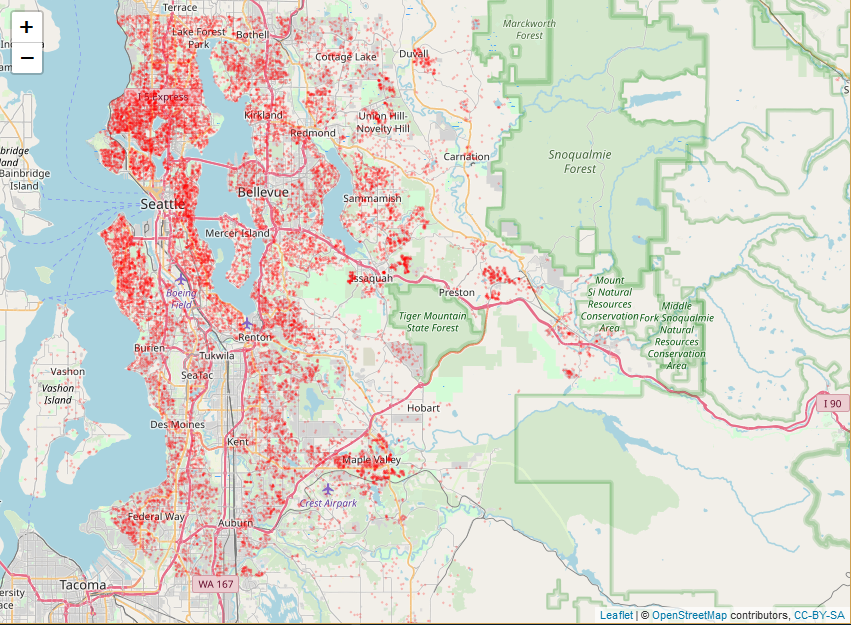
\includegraphics[width=450px]{King_county_map} \end{center}

\subsection{The variables}\label{the-variables}

Below is a description of each one of the variables available in the
data:

\begin{itemize}
\tightlist
\item
  id: Unique ID for each home sold
\item
  date: Date of the home sale
\item
  price: Price of each home sold
\item
  bedrooms: Number of bedrooms
\item
  bathrooms: Number of bathrooms, where .5 accounts for a room with a
  toilet but no shower
\item
  sqft\_living: Square footage of the apartments interior living space
\item
  sqft\_lot: Square footage of the land space
\item
  floors: Number of floors
\item
  waterfront: A dummy variable for whether the apartment was overlooking
  the waterfront or not
\item
  view: An index from 0 to 4 of how good the view of the property was
\item
  condition: An index from 1 to 5 on the condition of the apartment,
\item
  grade: An index from 1 to 13, where 1-3 falls short of building
  construction and design, 7 has an average level of construction and
  design, and 11-13 have a high quality level of construction and
  design.
\item
  sqft\_above: The square footage of the interior housing space that is
  above ground level
\item
  sqft\_basement: The square footage of the interior housing space that
  is below ground level
\item
  yr\_built: The year the house was initially built
\item
  yr\_renovated: The year of the house's last renovation
\item
  zipcode: What zipcode area the house is in
\item
  lat: Latitude
\item
  long: Longitude
\item
  sqft\_living15: The square footage of interior housing living space
  for the nearest 15 neighbors
\item
  sqft\_lot15: The square footage of the land lots of the nearest 15
  neighbors
\end{itemize}

\subsection{The response variable: numeric and visual
inspection}\label{the-response-variable-numeric-and-visual-inspection}

Here we observe some descriptive statistics about the sale prices:
\hfill\break

\begin{table}[H]
\centering
\begin{tabular}{r|r|r|r|r|r}
\hline
minimum & q1 & median & mean & q3 & maximum\\
\hline
75000 & 320000 & 450000 & 538212.5 & 641100 & 7700000\\
\hline
\end{tabular}
\end{table}

\hfill\break
By looking at the median and mean, we suspect skewness to the right in
the data. We verify this in the following visual inspection of the data:

\begin{center}\includegraphics{Report_files/figure-latex/unnamed-chunk-3-1} \end{center}

Additionally to confirming our suspicion of skewness to the right, we
observe in the qq-plot (the one on the right) that the distribution does
not fit the theoretical quantiles of the normal distribution. This goes
against the ``utopian'' assumption of normality for the response
variable when attempting linear regression analysis. \newpage
In order to improve this, we apply a simple transformation to the
response variable. The data is transformed to it's corresponding
logarithm with base 10. The following are the histogram and qq-plot of
the transformed variable:

\begin{center}\includegraphics{Report_files/figure-latex/unnamed-chunk-4-1} \end{center}

Although a perfect fit is difficult to achieve, the transformation
proves to be a huge improvement in terms of the normality assumption.

\subsection{The model selection}\label{the-model-selection}

In order to pick the best model, criteria must be specified. The p-value
presents the problem of multiple testing, and, since we will be
conducting several statistical tests, will only serve as a supporting
criteria.

Given this, the following metrics will be used for model comparison
instead:

\begin{itemize}
\tightlist
\item
  \(AIC\)
\item
  \(BIC\)
\item
  \(RMSE\)
\item
  \(T-Test\) \((p-value)\)
\end{itemize}

\subsubsection{The testing procedure}\label{the-testing-procedure}

The first model criteria we are considering are the AIC and the BIC.
Those are defined as:

\begin{align*}
    AIC &= -2logL(\hat{\theta}) + 2p \ & \ BIC &= -2logL(\hat{\theta}) + log(n)p\\
\end{align*}

The AIC is a model selection method which punishes the amount of
variables by adding two times the amount of variables to two times the
negative log likelihood of \(\hat{\theta}\), a lower value being the
desired outcome. Considering our data sets great amount of observations
(n = 21613) the punishment might be negligible. A better criterion might
therefore be the BIC which penalizes the amount of variables by
multiplying them with the log of the amount of observations. The BIC
will therefore be our preferred metric of those two. \newpage
Given that we are developing a predictive model, the most important
metric would still be the RMSE, the rooted mean square error, which is a
measure of the mean prediction error:

\begin{align*}
    RMSE &= \left(\sum_{i = 1}^{N} \left(y_{pi} - y_{oi}\right)^{2} \right)^{\frac{1}{2}}
\end{align*}

with:

\begin{itemize}
\tightlist
\item
  \(y_{pi}\) being the \(i\)-th predicted response value
\item
  \(y_{oi}\) being the \(i\)-th observed response value
\end{itemize}

This criterion gives us an actual predictive performance measurement to
compare different models against each other in a meaningful an easy to
interpret format, the amount of dollars for which a house was sold. To
make this metric and its comparisons even more precise we will use two
more different methods.

The first one will be a repeated cross-validation procedure using the
k-fold strategy. For this method the data set will be randomly divided
into \(k\) different folds. Leaving one fold out a model will be fitted
against the remaining folds. The model will then attempt to predict the
values of the fold previously left out and the RMSE will be calculated.
This procedure will be repeated for all the different folds. This whole
procedure of calculating the RMSE for all \(k\) folds will then again be
repeated for \(B\) times. In our case we will use \(k = 10\) and
\(B = 100\).

Using all those repeated measurements of the RMSE as a sample
distribution we are now able to use the second method of comparison, a
one sided two means t-test of the two RMSE distribution of two different
model. This gives us a measure of confidence, a p-value, about the
difference between those models.

\subsection{The a priori data
formating}\label{the-a-priori-data-formating}

It was necessary to do some initial formatting in order to make sense of
the data for a linear model. The modifications are the following:

\begin{itemize}
\tightlist
\item
  transforming square feet into square meters
\item
  converting waterfront, renovated and zipcode into factor variables
\item
  splitting date into week and month of the year, removing the original
  date variable
\item
  removing id because it is not informative
\item
  splitting dataset into two parts, 80\% and 20\% (the reserved part,
  more on this later) \hfill\break
\end{itemize}

\begin{Shaded}
\begin{Highlighting}[]
\NormalTok{full_data <-}\StringTok{ }\NormalTok{raw_data }\OperatorTok
\StringTok{  }\KeywordTok{mutate_at}\NormalTok{(}
    \KeywordTok{vars}\NormalTok{(}\KeywordTok{starts_with}\NormalTok{(}\StringTok{"sqft"}\NormalTok{)),}
    \ControlFlowTok{function}\NormalTok{(x) x }\OperatorTok{*}\StringTok{ }\FloatTok{0.092903}
\NormalTok{  ) }\OperatorTok
\StringTok{  }\KeywordTok{rename_at}\NormalTok{(}
    \KeywordTok{vars}\NormalTok{(}\KeywordTok{starts_with}\NormalTok{(}\StringTok{"sqft"}\NormalTok{)),}
    \ControlFlowTok{function}\NormalTok{(x) }\KeywordTok{str_replace}\NormalTok{(x, }\StringTok{"sqft"}\NormalTok{, }\StringTok{"sqm"}\NormalTok{)}
\NormalTok{  ) }\OperatorTok
\StringTok{  }\KeywordTok{mutate}\NormalTok{(}
    \DataTypeTok{week_of_year =} \KeywordTok{week}\NormalTok{(date),}
    \DataTypeTok{month_of_year =} \KeywordTok{month}\NormalTok{(date),}
    \DataTypeTok{renovated =} \KeywordTok{factor}\NormalTok{(}\KeywordTok{ifelse}\NormalTok{(yr_renovated }\OperatorTok{>}\StringTok{ }\DecValTok{0}\NormalTok{, }\StringTok{"yes"}\NormalTok{, }\StringTok{"no"}\NormalTok{)),}
    \DataTypeTok{wasViewed =} \KeywordTok{factor}\NormalTok{(}\KeywordTok{ifelse}\NormalTok{(view }\OperatorTok{>}\StringTok{ }\DecValTok{0}\NormalTok{, }\DecValTok{1}\NormalTok{, }\DecValTok{0}\NormalTok{)),}
    \DataTypeTok{waterfront =} \KeywordTok{factor}\NormalTok{(waterfront)}
\NormalTok{  ) }\OperatorTok
\StringTok{  }\KeywordTok{select}\NormalTok{(}\OperatorTok{-}\NormalTok{id, }\OperatorTok{-}\NormalTok{date, }\OperatorTok{-}\KeywordTok{starts_with}\NormalTok{(}\StringTok{"sqm"}\NormalTok{), }\KeywordTok{starts_with}\NormalTok{(}\StringTok{"sqm"}\NormalTok{))}

\NormalTok{first_fifth_avg <-}\StringTok{ }\NormalTok{data_20p }\OperatorTok
\StringTok{  }\KeywordTok{group_by}\NormalTok{(zipcode) }\OperatorTok
\StringTok{  }\KeywordTok{summarise}\NormalTok{(}\DataTypeTok{mean_price_zip =} \KeywordTok{mean}\NormalTok{(price))}

\NormalTok{full_data <-}\StringTok{ }\NormalTok{full_data }\OperatorTok
\StringTok{  }\KeywordTok{left_join}\NormalTok{(., first_fifth_avg, }\DataTypeTok{key =}\NormalTok{ zipcode) }\OperatorTok
\StringTok{  }\KeywordTok{mutate}\NormalTok{(}
    \DataTypeTok{price =} \KeywordTok{log10}\NormalTok{(price),}
    \DataTypeTok{mean_price_zip =} \KeywordTok{log10}\NormalTok{(mean_price_zip)}
\NormalTok{  )}
\end{Highlighting}
\end{Shaded}

\subsection{The first model}\label{the-first-model}

In the first model only the useful original variables will be included
with minimal formatting to provide a baseline for comparison.
\hfill\break

\begin{Shaded}
\begin{Highlighting}[]
\NormalTok{data_wo_new_vars <-}\StringTok{ }\NormalTok{full_data }\OperatorTok
\StringTok{  }\KeywordTok{select}\NormalTok{(}\OperatorTok{-}\NormalTok{wasViewed, }\OperatorTok{-}\NormalTok{renovated, }\OperatorTok{-}\NormalTok{mean_price_zip)}

\NormalTok{model_}\DecValTok{1}\NormalTok{ <-}\StringTok{ }\KeywordTok{lm}\NormalTok{(price }\OperatorTok{~}\StringTok{ }\NormalTok{., }\DataTypeTok{data =}\NormalTok{ data_wo_new_vars)}
\KeywordTok{summary}\NormalTok{(model_}\DecValTok{1}\NormalTok{)}
\end{Highlighting}
\end{Shaded}

\begin{verbatim}
## 
## Call:
## lm(formula = price ~ ., data = data_wo_new_vars)
## 
## Residuals:
##      Min       1Q   Median       3Q      Max 
## -0.79545 -0.06984  0.00137  0.06877  0.51844 
## 
## Coefficients: (1 not defined because of singularities)
##                    Estimate    Std. Error t value             Pr(>|t|)    
## (Intercept)   -1.0227807971  1.7821374985  -0.574              0.56604    
## bedrooms      -0.0065796282  0.0011934235  -5.513    0.000000035733833 ***
## bathrooms      0.0304110205  0.0019792560  15.365 < 0.0000000000000002 ***
## floors         0.0334927857  0.0021716861  15.422 < 0.0000000000000002 ***
## waterfront1    0.1657845101  0.0104082177  15.928 < 0.0000000000000002 ***
## view           0.0269147354  0.0013000536  20.703 < 0.0000000000000002 ***
## condition      0.0276373112  0.0014200196  19.463 < 0.0000000000000002 ***
## grade          0.0678112380  0.0013095874  51.781 < 0.0000000000000002 ***
## yr_built      -0.0014655209  0.0000439524 -33.343 < 0.0000000000000002 ***
## yr_renovated   0.0000165792  0.0000022486   7.373    0.000000000000174 ***
## zipcode       -0.0002920170  0.0000200183 -14.588 < 0.0000000000000002 ***
## lat            0.6089333776  0.0065181396  93.421 < 0.0000000000000002 ***
## long          -0.0682539439  0.0079122055  -8.626 < 0.0000000000000002 ***
## week_of_year  -0.0018685591  0.0006489327  -2.879              0.00399 ** 
## month_of_year  0.0057473400  0.0028245154   2.035              0.04189 *  
## sqm_living     0.0007156784  0.0000287739  24.872 < 0.0000000000000002 ***
## sqm_lot        0.0000021379  0.0000003206   6.668    0.000000000026751 ***
## sqm_above     -0.0000568279  0.0000285409  -1.991              0.04649 *  
## sqm_basement             NA            NA      NA                   NA    
## sqm_living15   0.0004488352  0.0000224319  20.009 < 0.0000000000000002 ***
## sqm_lot15     -0.0000012124  0.0000004785  -2.534              0.01130 *  
## ---
## Signif. codes:  0 '***' 0.001 '**' 0.01 '*' 0.05 '.' 0.1 ' ' 1
## 
## Residual standard error: 0.1092 on 17271 degrees of freedom
## Multiple R-squared:  0.7717, Adjusted R-squared:  0.7715 
## F-statistic:  3073 on 19 and 17271 DF,  p-value: < 0.00000000000000022
\end{verbatim}

\hfill\break
There are two peculiarities we can observe. In the first place, we
noticed the variable sqm\_basement was not taken into account and
consists solely of NAs. The second observation provides the reason for
this behavior: ``A singularity was discovered''. This means that
sqm\_basement is a linear combination of two or more other variables,
sqm\_living and sqm\_above in this case. The decision to remove those
variables will be dealt with during the experimentation phase.

\subsection{The experimentation
procedure}\label{the-experimentation-procedure}

Given that we now have both a baseline model and defined our model
selection criteria, using a trial and error approach, we can start
testing different approaches seeking to improve the model. Among those
approaches we will attempt outlier detection, creation of new and
meaningful variables, correlation analysis and different kinds of
variable transformations. Let us start with outlier detection.

\subsubsection{The outliers}\label{the-outliers}

Outliers, depending on their impact, may have a detrimental effect on
the capacity of a model to effectively fit itself to the general
patterns of the data and not just the present sample, which decreases
its predictive ability. To find those divergent data points we will have
a look at their leverage and the cook's distance.

\begin{itemize}
\tightlist
\item
  Leverage: The power to shift the model towards that specific data
  point
\end{itemize}

\begin{align*}
    h_i &= \frac{1}{n} + \frac{\left( x_i- \bar{x}\right)^{2}}{\sum_{i'=1}^{n} \left(x_{i'} - \bar{x} \right)^{2}}
\end{align*}

\begin{itemize}
\tightlist
\item
  Cook's distance: Measures the aggregated influence of that observation
  on the fitted values
\end{itemize}

\begin{align*}
    D_i &= \frac{E_{i}^{2}}{k+1} \cdot \frac{h_i}{1-h_i}
\end{align*}

\begin{Shaded}
\begin{Highlighting}[]
\KeywordTok{par}\NormalTok{(}\DataTypeTok{mfrow =} \KeywordTok{c}\NormalTok{(}\DecValTok{1}\NormalTok{,}\DecValTok{2}\NormalTok{))}
\KeywordTok{plot}\NormalTok{(model_}\DecValTok{1}\NormalTok{, }\DataTypeTok{which=}\DecValTok{5}\NormalTok{)}
\KeywordTok{plot}\NormalTok{(model_}\DecValTok{1}\NormalTok{, }\DataTypeTok{which=}\DecValTok{4}\NormalTok{)}
\end{Highlighting}
\end{Shaded}

\includegraphics{Report_files/figure-latex/unnamed-chunk-7-1.pdf}

Inspecting the cook's distance plot we find that there are 4 highly
influential data points. For the following test we will fit a linear
model without these aforementioned observations and compare it to our
baseline model. Note that in the following tables the p-value refers to
a one sided t-test of the model it is next to with the model directly
above. \hfill\break

\begin{Shaded}
\begin{Highlighting}[]
\NormalTok{full_data_woo <-}\StringTok{ }\NormalTok{full_data }\OperatorTok
\StringTok{  }\CommentTok{#select(-wasViewed, -renovated, -mean_price_zip) %>%}
\StringTok{  }\KeywordTok{slice}\NormalTok{(}\KeywordTok{c}\NormalTok{(}\OperatorTok{-}\DecValTok{11520}\NormalTok{, }\OperatorTok{-}\DecValTok{3183}\NormalTok{, }\OperatorTok{-}\DecValTok{6187}\NormalTok{, }\OperatorTok{-}\DecValTok{8844}\NormalTok{))}

\NormalTok{cross_val <-}\StringTok{ }\ControlFlowTok{function}\NormalTok{(data, }\DataTypeTok{B =} \DecValTok{100}\NormalTok{, }\DataTypeTok{k =} \DecValTok{10}\NormalTok{)\{}
\NormalTok{  n <-}\StringTok{ }\KeywordTok{nrow}\NormalTok{(data)}
\NormalTok{  folds <-}\StringTok{ }\KeywordTok{sample}\NormalTok{(}\KeywordTok{rep}\NormalTok{(}\KeywordTok{c}\NormalTok{(}\DecValTok{1}\OperatorTok{:}\NormalTok{k), }\DataTypeTok{length.out =} \KeywordTok{nrow}\NormalTok{(data)))}
\NormalTok{  results <-}\StringTok{ }\KeywordTok{foreach}\NormalTok{(}\KeywordTok{icount}\NormalTok{(B), }\DataTypeTok{.combine =}\NormalTok{ cbind) }\OperatorTok\StringTok{ }\NormalTok{\{}
\NormalTok{    res <-}\StringTok{ }\KeywordTok{numeric}\NormalTok{(k)}
    \ControlFlowTok{for}\NormalTok{ (i }\ControlFlowTok{in} \DecValTok{1}\OperatorTok{:}\NormalTok{k) \{}
\NormalTok{      training <-}\StringTok{ }\NormalTok{data[folds }\OperatorTok{!=}\StringTok{ }\NormalTok{i,]}
\NormalTok{      test <-}\StringTok{ }\NormalTok{data[folds }\OperatorTok{==}\StringTok{ }\NormalTok{i,]}

\NormalTok{      lmo <-}\StringTok{ }\KeywordTok{lm}\NormalTok{(}\DataTypeTok{data =}\NormalTok{ training, price }\OperatorTok{~}\StringTok{ }\NormalTok{.)}
\NormalTok{      predict <-}\StringTok{ }\KeywordTok{predict}\NormalTok{(lmo, test)}
    
\NormalTok{      res[i] <-}\StringTok{ }\KeywordTok{sum}\NormalTok{((}\DecValTok{10}\OperatorTok{^}\NormalTok{test}\OperatorTok{$}\NormalTok{price }\OperatorTok{-}\StringTok{ }\DecValTok{10}\OperatorTok{^}\NormalTok{predict)}\OperatorTok{^}\DecValTok{2}\NormalTok{)}\OperatorTok{/}\KeywordTok{length}\NormalTok{(test}\OperatorTok{$}\NormalTok{price)}
\NormalTok{    \}}
\NormalTok{    res}
\NormalTok{  \}}
\NormalTok{  m_rmse <-}\StringTok{ }\KeywordTok{mean}\NormalTok{(}\KeywordTok{sqrt}\NormalTok{(results))}
\NormalTok{  sd_rmse <-}\StringTok{ }\KeywordTok{sd}\NormalTok{(}\KeywordTok{sqrt}\NormalTok{(results))}
\NormalTok{  l <-}\StringTok{ }\KeywordTok{list}\NormalTok{(}\DataTypeTok{distr =} \KeywordTok{sqrt}\NormalTok{(results), }\DataTypeTok{m_rmse =}\NormalTok{ m_rmse, }\DataTypeTok{sd_rmse =}\NormalTok{ sd_rmse)}
  \KeywordTok{return}\NormalTok{(l)}
\NormalTok{\}}

\NormalTok{intermediate_}\DecValTok{1}\NormalTok{ <-}\StringTok{ }\NormalTok{full_data_woo }\OperatorTok
\StringTok{  }\KeywordTok{select}\NormalTok{(}\OperatorTok{-}\NormalTok{wasViewed, }\OperatorTok{-}\NormalTok{renovated, }\OperatorTok{-}\NormalTok{mean_price_zip)}

\NormalTok{intermediate_}\DecValTok{2}\NormalTok{ <-}\StringTok{ }\NormalTok{data_wo_new_vars}

\NormalTok{model_}\DecValTok{2}\NormalTok{ <-}\StringTok{ }\NormalTok{intermediate_}\DecValTok{1} \OperatorTok
\StringTok{  }\KeywordTok{lm}\NormalTok{(}\DataTypeTok{data =}\NormalTok{ . , price }\OperatorTok{~}\StringTok{ }\NormalTok{.)}

\NormalTok{cv_}\DecValTok{2}\NormalTok{ <-}\StringTok{ }\KeywordTok{cross_val}\NormalTok{(intermediate_}\DecValTok{1}\NormalTok{)}
\NormalTok{cv_}\DecValTok{1}\NormalTok{ <-}\StringTok{ }\KeywordTok{cross_val}\NormalTok{(intermediate_}\DecValTok{2}\NormalTok{)}

\NormalTok{p_value_}\DecValTok{1}\NormalTok{ <-}\StringTok{ }
\StringTok{  }\KeywordTok{tidy}\NormalTok{(}\KeywordTok{t.test}\NormalTok{(cv_}\DecValTok{1}\OperatorTok{$}\NormalTok{distr, cv_}\DecValTok{2}\OperatorTok{$}\NormalTok{distr, }\DataTypeTok{var.equal =}\NormalTok{ F, }\DataTypeTok{alternative =} \StringTok{"greater"}\NormalTok{)) }\OperatorTok\StringTok{ }
\StringTok{  }\KeywordTok{select}\NormalTok{(p.value) }\OperatorTok\StringTok{ }
\StringTok{  }\KeywordTok{unlist}\NormalTok{() }\OperatorTok\StringTok{ }
\StringTok{  }\KeywordTok{formatC}\NormalTok{(}\DataTypeTok{format =} \StringTok{"e"}\NormalTok{) }\OperatorTok\StringTok{ }
\StringTok{  }\KeywordTok{rbind}\NormalTok{(}\StringTok{" "}\NormalTok{,.)}

\NormalTok{Mean_RMSE <-}\StringTok{ }\KeywordTok{round}\NormalTok{(}\KeywordTok{rbind}\NormalTok{(cv_}\DecValTok{1}\OperatorTok{$}\NormalTok{m_rmse, cv_}\DecValTok{2}\OperatorTok{$}\NormalTok{m_rmse), }\DecValTok{0}\NormalTok{)}
\NormalTok{SD_RMSE <-}\StringTok{ }\KeywordTok{round}\NormalTok{(}\KeywordTok{rbind}\NormalTok{(cv_}\DecValTok{1}\OperatorTok{$}\NormalTok{sd_rmse, cv_}\DecValTok{2}\OperatorTok{$}\NormalTok{sd_rmse), }\DecValTok{0}\NormalTok{)}

\KeywordTok{cbind}\NormalTok{(}\KeywordTok{BIC}\NormalTok{(model_}\DecValTok{1}\NormalTok{, model_}\DecValTok{2}\NormalTok{), Mean_RMSE, SD_RMSE, p_value_}\DecValTok{1}\NormalTok{) }\OperatorTok
\StringTok{  }\KeywordTok{kable}\NormalTok{() }\OperatorTok\StringTok{ }
\StringTok{  }\KeywordTok{kable_styling}\NormalTok{()}
\end{Highlighting}
\end{Shaded}

\begin{table}[H]
\centering
\begin{tabular}{l|r|r|r|r|l}
\hline
  & df & BIC & Mean\_RMSE & SD\_RMSE & p.value\\
\hline
model\_1 & 21 & -27338.06 & 203777 & 56684 & \\
\hline
model\_2 & 21 & -27420.96 & 186945 & 30079 & 1.1816e-16\\
\hline
\end{tabular}
\end{table}

\hfill\break
Out of the resulting summary table, we can draw some conclusions
regarding the removal of these outliers:

\begin{itemize}
\tightlist
\item
  By solely looking at the three first metrics (AIC, mean of RMSE and
  s.d. of RMSE) we can see that removal of outliers proved to be
  successful.
\item
  When looking only at the mean RMSE, we observe it was reduced by about
  20.000\$. This, in terms of usefulness as a prediction tool in real
  life scenarios, is very desirable, given that it provides the end user
  with a more accurate estimation of the actual values.
\item
  The standard deviation of RMSE errors was cut almost by half, meaning
  that the new models are way more stable.
\item
  The last metric of the table, the p-value, verifies the significance
  of the conclusions made above. Since the resulting number is very low
  (highly significant), we proceed to conclude with enough confidence
  (\textgreater{}99\%) that the previous statements are valid.
\item
  The BIC was reduced by 83.
\end{itemize}

In terms of data points (observations) there will be no further
additions or removals from now on. So, the next phases of
experimentation, are rather column-wise, and focus on the creation,
deletion or edition of the variables as a whole.

\subsubsection{The creating of new
variables}\label{the-creating-of-new-variables}

In this phase we decided to create some additional variables by using
some the reserved part of the data in the current ones or by creating a
simplified version of an existing one.

\paragraph{\texorpdfstring{The ``Average price by zipcode''
variable:}{The Average price by zipcode variable:}}\label{the-average-price-by-zipcode-variable}

To understand the creation process of this variable and why it is a
valid thing to do, it is necessary to explain the 80\%-20\% data
splitting mentioned before in the \emph{Preliminary data formating}
section.

It goes as follows: Since the split of the data, made at the very
beginning, we have only worked with the 80\% chunk, which comes to
represent the only usable data for our experiments, model comparison,
conclusion making and everything else. Given this, we could see the rest
of the 20\% data as ``preconceived''. By doing so, we intend to pretend
as if the information (including the sale prices) provided by this
usable set of observations is available throughout all the study. It is
not considered data leakage since the rows themselves are not being used
to train or evaluate any model at any point.

So, how are we utilizing this data exactly? By using them as a summary
of prices by zipcode. First we select the zipcode and the price columns
in this 20\% chunk, then we group the observations by their zipcode and
compute the average price within each zipcode. Finally in the 80\% data
chunk, we create a new column containing the average price found in the
corresponding zipcode-price pairs obtained with the 20\% chunk. In this
way, we have obtained additional data to the model, which is related to
the prices, without falling prey to data leakage. \hfill\break

\begin{Shaded}
\begin{Highlighting}[]
\NormalTok{intermediate_}\DecValTok{3}\NormalTok{ <-}\StringTok{ }\NormalTok{full_data_woo }\OperatorTok\StringTok{ }
\StringTok{  }\KeywordTok{select}\NormalTok{(}\OperatorTok{-}\NormalTok{wasViewed, }\OperatorTok{-}\NormalTok{renovated)}

\NormalTok{model_}\DecValTok{3}\NormalTok{ <-}\StringTok{ }\KeywordTok{lm}\NormalTok{(price }\OperatorTok{~}\StringTok{ }\NormalTok{., }\DataTypeTok{data =}\NormalTok{ intermediate_}\DecValTok{3}\NormalTok{)}

\NormalTok{cv_}\DecValTok{3}\NormalTok{ <-}\StringTok{ }\KeywordTok{cross_val}\NormalTok{(intermediate_}\DecValTok{3}\NormalTok{)}

\NormalTok{p_value_}\DecValTok{2}\NormalTok{ <-}\StringTok{ }
\StringTok{  }\KeywordTok{tidy}\NormalTok{(}\KeywordTok{t.test}\NormalTok{(cv_}\DecValTok{2}\OperatorTok{$}\NormalTok{distr, cv_}\DecValTok{3}\OperatorTok{$}\NormalTok{distr, }\DataTypeTok{var.equal =}\NormalTok{ F, }\DataTypeTok{alternative =} \StringTok{"greater"}\NormalTok{)) }\OperatorTok\StringTok{ }
\StringTok{  }\KeywordTok{select}\NormalTok{(p.value) }\OperatorTok\StringTok{ }
\StringTok{  }\KeywordTok{unlist}\NormalTok{() }\OperatorTok\StringTok{ }
\StringTok{  }\KeywordTok{formatC}\NormalTok{(}\DataTypeTok{format =} \StringTok{"e"}\NormalTok{)}

\NormalTok{Mean_RMSE <-}\StringTok{ }\KeywordTok{round}\NormalTok{(}\KeywordTok{rbind}\NormalTok{(cv_}\DecValTok{2}\OperatorTok{$}\NormalTok{m_rmse, cv_}\DecValTok{3}\OperatorTok{$}\NormalTok{m_rmse))}
\NormalTok{SD_RMSE <-}\StringTok{ }\KeywordTok{round}\NormalTok{(}\KeywordTok{rbind}\NormalTok{(cv_}\DecValTok{2}\OperatorTok{$}\NormalTok{sd_rmse, cv_}\DecValTok{3}\OperatorTok{$}\NormalTok{sd_rmse))}
\NormalTok{p_vals <-}\StringTok{ }\KeywordTok{rbind}\NormalTok{(}\StringTok{" "}\NormalTok{, p_value_}\DecValTok{2}\NormalTok{)}

\KeywordTok{cbind}\NormalTok{(}\KeywordTok{BIC}\NormalTok{(model_}\DecValTok{2}\NormalTok{, model_}\DecValTok{3}\NormalTok{), Mean_RMSE, SD_RMSE, p_vals) }\OperatorTok
\StringTok{  }\KeywordTok{kable}\NormalTok{() }\OperatorTok\StringTok{ }
\StringTok{  }\KeywordTok{kable_styling}\NormalTok{()}
\end{Highlighting}
\end{Shaded}

\begin{table}[H]
\centering
\begin{tabular}{l|r|r|r|r|l}
\hline
  & df & BIC & Mean\_RMSE & SD\_RMSE & p.value\\
\hline
model\_2 & 21 & -27420.96 & 186945 & 30079 & \\
\hline
model\_3 & 22 & -35341.87 & 155384 & 35346 & 1.6393e-92\\
\hline
\end{tabular}
\end{table}

\hfill\break
Once again, let us analyze the resulting summary:

\begin{itemize}
\tightlist
\item
  In terms of our comparison criteria, introducing this new variables
  improves the model.
\item
  The mean RMSE is reduced by about 30.000\$
\item
  The standard deviation of the RMSE remains similar to the previous
  one. So adding this variable does not destabilizes the model
  considerably.
\item
  Once again, the p-value obtained suggests that the difference in the
  distribution of RMSEs is highly significant when using this additional
  variable.
\item
  Considerably large improvement in the BIC metric. \newpage
\end{itemize}

\paragraph{The factorization:}\label{the-factorization}

The second and third additional columns are less complicated, being only
a simplification of two current columns. The general reasoning is rather
than using all the values provided in the column, we are only concerned
on whether or not there is a non-zero value present. The specific
transformations are:

\begin{itemize}
\tightlist
\item
  From the \emph{view} variable, create a ``yes or no'' variable
  indicating if the properties has been viewed or not.
\item
  From the \emph{year renovated} variable, create a variable that
  specifies if the property has ever been renovated or not.
\end{itemize}

For the following experiment, we will test if adding the transformed
variables will improve the model as well as whether we should keep the
untransformed original ones on which the new ones are based or not. Note
that in the following output the p-value always refers to a comparison
against the uppermost model within the table. \hfill\break

\begin{Shaded}
\begin{Highlighting}[]
\NormalTok{intermediate_}\FloatTok{3.1}\NormalTok{ <-}\StringTok{ }\NormalTok{full_data_woo}
\NormalTok{model_}\FloatTok{3.1}\NormalTok{ <-}\StringTok{ }\KeywordTok{lm}\NormalTok{(price }\OperatorTok{~}\StringTok{ }\NormalTok{., }\DataTypeTok{data =}\NormalTok{ intermediate_}\FloatTok{3.1}\NormalTok{)}

\NormalTok{cv_}\FloatTok{3.1}\NormalTok{ <-}\StringTok{ }\KeywordTok{cross_val}\NormalTok{(intermediate_}\FloatTok{3.1}\NormalTok{)}

\NormalTok{p_value_}\FloatTok{2.1}\NormalTok{ <-}\StringTok{ }
\StringTok{  }\KeywordTok{tidy}\NormalTok{(}\KeywordTok{t.test}\NormalTok{(cv_}\DecValTok{3}\OperatorTok{$}\NormalTok{distr, cv_}\FloatTok{3.1}\OperatorTok{$}\NormalTok{distr, }\DataTypeTok{var.equal =}\NormalTok{ F, }\DataTypeTok{alternative =} \StringTok{"greater"}\NormalTok{)) }\OperatorTok\StringTok{ }
\StringTok{  }\KeywordTok{select}\NormalTok{(p.value) }\OperatorTok\StringTok{ }
\StringTok{  }\KeywordTok{unlist}\NormalTok{() }\OperatorTok\StringTok{ }
\StringTok{  }\KeywordTok{round}\NormalTok{(., }\DecValTok{2}\NormalTok{)}

\NormalTok{intermediate_}\FloatTok{3.2}\NormalTok{ <-}\StringTok{ }\NormalTok{full_data_woo }\OperatorTok\StringTok{ }
\StringTok{  }\KeywordTok{select}\NormalTok{(}\OperatorTok{-}\NormalTok{view, }\OperatorTok{-}\NormalTok{yr_renovated)}

\NormalTok{model_}\FloatTok{3.2}\NormalTok{ <-}\StringTok{ }\KeywordTok{lm}\NormalTok{(price }\OperatorTok{~}\StringTok{ }\NormalTok{., }\DataTypeTok{data =}\NormalTok{ intermediate_}\FloatTok{3.2}\NormalTok{)}

\NormalTok{cv_}\FloatTok{3.2}\NormalTok{ <-}\StringTok{ }\KeywordTok{cross_val}\NormalTok{(intermediate_}\FloatTok{3.2}\NormalTok{)}

\NormalTok{p_value_}\FloatTok{2.2}\NormalTok{ <-}\StringTok{ }
\StringTok{  }\KeywordTok{tidy}\NormalTok{(}\KeywordTok{t.test}\NormalTok{(cv_}\DecValTok{3}\OperatorTok{$}\NormalTok{distr, cv_}\FloatTok{3.2}\OperatorTok{$}\NormalTok{distr, }\DataTypeTok{var.equal =}\NormalTok{ F, }\DataTypeTok{alternative =} \StringTok{"greater"}\NormalTok{)) }\OperatorTok\StringTok{ }
\StringTok{  }\KeywordTok{select}\NormalTok{(p.value) }\OperatorTok\StringTok{ }
\StringTok{  }\KeywordTok{unlist}\NormalTok{() }\OperatorTok\StringTok{ }
\StringTok{  }\KeywordTok{round}\NormalTok{(., }\DecValTok{2}\NormalTok{)}

\NormalTok{Mean_RMSE <-}\StringTok{ }\KeywordTok{round}\NormalTok{(}\KeywordTok{rbind}\NormalTok{(cv_}\DecValTok{3}\OperatorTok{$}\NormalTok{m_rmse, cv_}\FloatTok{3.1}\OperatorTok{$}\NormalTok{m_rmse, cv_}\FloatTok{3.2}\OperatorTok{$}\NormalTok{m_rmse))}
\NormalTok{SD_RMSE <-}\StringTok{ }\KeywordTok{round}\NormalTok{(}\KeywordTok{rbind}\NormalTok{(cv_}\DecValTok{3}\OperatorTok{$}\NormalTok{sd_rmse, cv_}\FloatTok{3.1}\OperatorTok{$}\NormalTok{sd_rmse, cv_}\FloatTok{3.2}\OperatorTok{$}\NormalTok{sd_rmse))}
\NormalTok{p_vals <-}\StringTok{ }\KeywordTok{rbind}\NormalTok{(}\StringTok{" "}\NormalTok{, p_value_}\FloatTok{2.1}\NormalTok{, p_value_}\FloatTok{2.2}\NormalTok{)}

\KeywordTok{cbind}\NormalTok{(}\KeywordTok{BIC}\NormalTok{(model_}\DecValTok{3}\NormalTok{, model_}\FloatTok{3.1}\NormalTok{, model_}\FloatTok{3.2}\NormalTok{), Mean_RMSE, SD_RMSE, p_vals) }\OperatorTok
\StringTok{  }\KeywordTok{kable}\NormalTok{() }\OperatorTok\StringTok{ }
\StringTok{  }\KeywordTok{kable_styling}\NormalTok{()}
\end{Highlighting}
\end{Shaded}

\begin{table}[H]
\centering
\begin{tabular}{l|r|r|r|r|l}
\hline
  & df & BIC & Mean\_RMSE & SD\_RMSE & p.value\\
\hline
model\_3 & 22 & -35341.87 & 155384 & 35346 & \\
\hline
model\_3.1 & 24 & -35391.64 & 154127 & 28181 & 0.19\\
\hline
model\_3.2 & 22 & -35296.07 & 155212 & 25355 & 0.45\\
\hline
\end{tabular}
\end{table}

\hfill\break
As the tests reveal, keeping the factorized variables while removing the
variables they are based on (model 3.2) proved to be of no improvement
at all. If anything it decreases the accuracy in terms of the BIC.

On the other hand factorizing while keeping the original variables
(model 3.1) improves the model performance slightly as indicated by the
drop in BIC of about 50 points. The mean RMSE was reduced to some extent
as well, although the p-value indicates a low chance of this difference
being significant.

Now that we have attempted and tested creations of new variables, we'll
proceed with correlation analysis in the next section. Although our
experiments so far suggest that at least one of the recently added
variables will stay present in the final model, given the improvements
obtained when adding the three of them, they are still subject to
testing.

\subsubsection{The correlation analysis}\label{the-correlation-analysis}

In the following table, we present the correlation coefficients between
each of the predictors and the target variable (price). The idea is to
determine how linearly related are each of those variables to the
response and based on this, do a sub selection of the most correlated
ones to determine if there is an improvement. \hfill\break

\begin{table}[H]
\centering
\begin{tabular}{l|l|l|l|l|l}
\hline
month\_of\_year & 0.0174 & sqm\_lot & 0.0962 & bathrooms & 0.5508\\
\hline
week\_of\_year & 0.0197 & yr\_renovated & 0.1074 & sqm\_above & 0.602\\
\hline
zipcode & 0.0372 & floors & 0.314 & sqm\_living15 & 0.6187\\
\hline
condition & 0.0396 & sqm\_basement & 0.3191 & sqm\_living & 0.6945\\
\hline
long & 0.0485 & bedrooms & 0.3489 & grade & 0.7022\\
\hline
yr\_built & 0.0826 & view & 0.3504 & mean\_price\_zip & 0.7172\\
\hline
sqm\_lot15 & 0.0909 & lat & 0.4482 & price & 1\\
\hline
\end{tabular}
\end{table}

\hfill\break
Looking at the table, we suggest the following hypothesis: Given that we
observe a big jump in correlation from 0.107 to 0.314 in between the
variable yr\_renovated and floor, dropping all variables with a
correlation below 0.314 might decrease prediction error and improve the
model. \hfill\break

\begin{Shaded}
\begin{Highlighting}[]
\NormalTok{intermediate_}\DecValTok{4}\NormalTok{ <-}\StringTok{ }\NormalTok{full_data_woo }\OperatorTok
\StringTok{  }\NormalTok{dplyr}\OperatorTok{::}\KeywordTok{select}\NormalTok{(}\KeywordTok{one_of}\NormalTok{(good_corr), waterfront)}

\NormalTok{model_}\DecValTok{4}\NormalTok{ <-}\StringTok{ }\KeywordTok{lm}\NormalTok{(price }\OperatorTok{~}\StringTok{ }\NormalTok{., }\DataTypeTok{data =}\NormalTok{ intermediate_}\DecValTok{4}\NormalTok{)}

\NormalTok{cv_}\DecValTok{4}\NormalTok{ <-}\StringTok{ }\KeywordTok{cross_val}\NormalTok{(intermediate_}\DecValTok{4}\NormalTok{)}

\NormalTok{Mean_RMSE <-}\StringTok{ }\KeywordTok{round}\NormalTok{(}\KeywordTok{rbind}\NormalTok{(cv_}\DecValTok{3}\OperatorTok{$}\NormalTok{m_rmse, cv_}\DecValTok{4}\OperatorTok{$}\NormalTok{m_rmse), }\DecValTok{0}\NormalTok{)}
\NormalTok{SD_RMSE <-}\StringTok{ }\KeywordTok{round}\NormalTok{(}\KeywordTok{rbind}\NormalTok{(cv_}\DecValTok{3}\OperatorTok{$}\NormalTok{sd_rmse, cv_}\DecValTok{4}\OperatorTok{$}\NormalTok{sd_rmse), }\DecValTok{0}\NormalTok{)}

\NormalTok{p_value_}\DecValTok{3}\NormalTok{ <-}\StringTok{ }
\StringTok{  }\KeywordTok{tidy}\NormalTok{(}\KeywordTok{t.test}\NormalTok{(cv_}\DecValTok{3}\OperatorTok{$}\NormalTok{distr, cv_}\DecValTok{4}\OperatorTok{$}\NormalTok{distr, }\DataTypeTok{var.equal =}\NormalTok{ F, }\DataTypeTok{alternative =} \StringTok{"greater"}\NormalTok{)) }\OperatorTok\StringTok{ }
\StringTok{  }\KeywordTok{select}\NormalTok{(p.value) }\OperatorTok\StringTok{ }
\StringTok{  }\KeywordTok{unlist}\NormalTok{() }\OperatorTok\StringTok{ }
\StringTok{  }\KeywordTok{round}\NormalTok{(., }\DecValTok{2}\NormalTok{) }\OperatorTok\StringTok{ }
\StringTok{  }\KeywordTok{rbind}\NormalTok{(}\StringTok{" "}\NormalTok{,.)}

\KeywordTok{cbind}\NormalTok{(}\KeywordTok{BIC}\NormalTok{(model_}\DecValTok{3}\NormalTok{, model_}\DecValTok{4}\NormalTok{), Mean_RMSE, SD_RMSE, p_value_}\DecValTok{3}\NormalTok{) }\OperatorTok
\StringTok{  }\KeywordTok{kable}\NormalTok{() }\OperatorTok\StringTok{ }
\StringTok{  }\KeywordTok{kable_styling}\NormalTok{()}
\end{Highlighting}
\end{Shaded}

\begin{table}[H]
\centering
\begin{tabular}{l|r|r|r|r|l}
\hline
  & df & BIC & Mean\_RMSE & SD\_RMSE & p.value\\
\hline
model\_3 & 22 & -35341.87 & 155384 & 35346 & \\
\hline
model\_4 & 13 & -33124.77 & 159525 & 23983 & 1\\
\hline
\end{tabular}
\end{table}

As we can see, although the variability of the predictions is reduced,
the actual mean of the RMSEs increases, which is not a desirable result.
This together with the huge increase of the BIC, dropping the less
correlated variables decreases the model performance. Looking at the
p-value, we realize that there is no evidence at all that the reduced
model performs better.

\subsubsection{The variable selection}\label{the-variable-selection}

As we saw earlier the variable sqm\_living is a linear combination of
sqm\_above and sqm\_basement. Thus it might be reasonable to select the
best performing model with a certain subset of those variables. To
figure that out we first tried to find the best transformation of the
all of those variables under the assumption that doing so might improve
the RMSE. We used an array of different transformations for each
variable separately and evaluated the impact through the change in the
BIC compared to a model containing the untransformed variable.
\hfill\break

\begin{Shaded}
\begin{Highlighting}[]
\NormalTok{intermediate_}\DecValTok{5}\NormalTok{ <-}\StringTok{ }\NormalTok{full_data_woo }\OperatorTok
\StringTok{  }\KeywordTok{mutate}\NormalTok{(}
    \DataTypeTok{sqm_above =} \KeywordTok{sqrt}\NormalTok{(sqm_above),}
    \DataTypeTok{sqm_basement =} \KeywordTok{sqrt}\NormalTok{(sqm_basement)}
\NormalTok{    ) }\OperatorTok\StringTok{ }
\StringTok{  }\NormalTok{dplyr}\OperatorTok{::}\KeywordTok{select}\NormalTok{(}\OperatorTok{-}\NormalTok{sqm_living)}

\NormalTok{model_}\DecValTok{5}\NormalTok{ <-}\StringTok{ }\KeywordTok{lm}\NormalTok{(}\DataTypeTok{data =}\NormalTok{ intermediate_}\DecValTok{5}\NormalTok{, price }\OperatorTok{~}\StringTok{ }\NormalTok{.)}

\NormalTok{intermediate_}\DecValTok{6}\NormalTok{ <-}\StringTok{ }\NormalTok{full_data_woo }\OperatorTok
\StringTok{  }\KeywordTok{mutate_at}\NormalTok{(}\KeywordTok{vars}\NormalTok{(sqm_living), sqrt) }\OperatorTok
\StringTok{  }\NormalTok{dplyr}\OperatorTok{::}\KeywordTok{select}\NormalTok{(}\OperatorTok{-}\NormalTok{sqm_above, }\OperatorTok{-}\NormalTok{sqm_basement) }

\NormalTok{model_}\DecValTok{6}\NormalTok{ <-}\StringTok{ }\KeywordTok{lm}\NormalTok{(}\DataTypeTok{data =}\NormalTok{ intermediate_}\DecValTok{6}\NormalTok{, price }\OperatorTok{~}\StringTok{ }\NormalTok{.)}

\NormalTok{s_model_}\DecValTok{5}\NormalTok{ <-}\StringTok{ }\KeywordTok{summary}\NormalTok{(model_}\DecValTok{5}\NormalTok{)}
\NormalTok{s_model_}\DecValTok{6}\NormalTok{ <-}\StringTok{ }\KeywordTok{summary}\NormalTok{(model_}\DecValTok{6}\NormalTok{)}

\NormalTok{cv_}\DecValTok{5}\NormalTok{ <-}\StringTok{ }\KeywordTok{cross_val}\NormalTok{(intermediate_}\DecValTok{5}\NormalTok{)}
\NormalTok{cv_}\DecValTok{6}\NormalTok{ <-}\StringTok{ }\KeywordTok{cross_val}\NormalTok{(intermediate_}\DecValTok{6}\NormalTok{)}

\NormalTok{p_value_}\DecValTok{4}\NormalTok{ <-}\StringTok{ }\KeywordTok{tidy}\NormalTok{(}\KeywordTok{t.test}\NormalTok{(cv_}\DecValTok{5}\OperatorTok{$}\NormalTok{distr, cv_}\DecValTok{6}\OperatorTok{$}\NormalTok{distr, }\DataTypeTok{var.equal =}\NormalTok{ F)) }\OperatorTok\StringTok{ }
\StringTok{  }\KeywordTok{select}\NormalTok{(p.value) }\OperatorTok\StringTok{ }
\StringTok{  }\KeywordTok{unlist}\NormalTok{()}

\NormalTok{row_names <-}\StringTok{ }\KeywordTok{c}\NormalTok{(}\StringTok{"above & basement"}\NormalTok{, }\StringTok{"living"}\NormalTok{)}
\NormalTok{col_names <-}\StringTok{ }\KeywordTok{c}\NormalTok{(}\StringTok{"R^2 adjust."}\NormalTok{, }\StringTok{"AIC"}\NormalTok{, }\StringTok{"BIC"}\NormalTok{, }\StringTok{"Mean_RMSE"}\NormalTok{, }\StringTok{"SD_RMSE"}\NormalTok{, }\StringTok{"P-value"}\NormalTok{)}
\NormalTok{a <-}\StringTok{ }\KeywordTok{matrix}\NormalTok{(}
  \KeywordTok{c}\NormalTok{(}
    \KeywordTok{round}\NormalTok{(s_model_}\DecValTok{5}\OperatorTok{$}\NormalTok{adj.r.squared, }\DecValTok{4}\NormalTok{),}
    \KeywordTok{round}\NormalTok{(}\KeywordTok{AIC}\NormalTok{(model_}\DecValTok{5}\NormalTok{), }\DecValTok{0}\NormalTok{),}
    \KeywordTok{round}\NormalTok{(}\KeywordTok{BIC}\NormalTok{(model_}\DecValTok{5}\NormalTok{), }\DecValTok{0}\NormalTok{),}
    \KeywordTok{round}\NormalTok{(cv_}\DecValTok{5}\OperatorTok{$}\NormalTok{m_rmse, }\DecValTok{0}\NormalTok{),}
    \KeywordTok{round}\NormalTok{(cv_}\DecValTok{5}\OperatorTok{$}\NormalTok{sd_rmse, }\DecValTok{0}\NormalTok{),}
    \StringTok{" "}\NormalTok{,}
    \KeywordTok{round}\NormalTok{(s_model_}\DecValTok{6}\OperatorTok{$}\NormalTok{adj.r.squared, }\DecValTok{4}\NormalTok{),}
    \KeywordTok{round}\NormalTok{(}\KeywordTok{AIC}\NormalTok{(model_}\DecValTok{6}\NormalTok{), }\DecValTok{0}\NormalTok{),}
    \KeywordTok{round}\NormalTok{(}\KeywordTok{BIC}\NormalTok{(model_}\DecValTok{6}\NormalTok{), }\DecValTok{0}\NormalTok{),}
    \KeywordTok{round}\NormalTok{(cv_}\DecValTok{6}\OperatorTok{$}\NormalTok{m_rmse, }\DecValTok{0}\NormalTok{),}
    \KeywordTok{round}\NormalTok{(cv_}\DecValTok{6}\OperatorTok{$}\NormalTok{sd_rmse, }\DecValTok{0}\NormalTok{),}
    \KeywordTok{round}\NormalTok{(p_value_}\DecValTok{4}\NormalTok{, }\DecValTok{2}\NormalTok{)),}
  \DataTypeTok{ncol =} \DecValTok{6}\NormalTok{,}
  \DataTypeTok{byrow =}\NormalTok{ T,}
  \DataTypeTok{dimnames =} \KeywordTok{list}\NormalTok{(row_names, col_names)}
\NormalTok{)}

\NormalTok{a }\OperatorTok
\StringTok{  }\KeywordTok{kable}\NormalTok{() }\OperatorTok\StringTok{ }
\StringTok{  }\KeywordTok{kable_styling}\NormalTok{()}
\end{Highlighting}
\end{Shaded}

\begin{table}[H]
\centering
\begin{tabular}{l|l|l|l|l|l|l}
\hline
  & R\textasciicircum{}2 adjust. & AIC & BIC & Mean\_RMSE & SD\_RMSE & P-value\\
\hline
above \& basement & 0.8606 & -36049 & -35863 & 133703 & 9328 & \\
\hline
living & 0.86 & -35976 & -35798 & 134038 & 6253 & 0.35\\
\hline
\end{tabular}
\end{table}

\hfill\break
Comparing both models with each other the result is quite inconclusive.
On the one hand, the p-value indicates that there is no significant
difference between their distributions of RMSEs. According to the
principle of parsimony one should stick with the second model,
containing sqm\_living instead of sqm\_basement and sqm\_above, due to a
reduced amount of variables.

However the BIC, AIC and the adjusted \(R^2\) suggest the first model to
be the more precise one and that's why we have chosen to stick to this
particular model.

\subsubsection{The reduced model}\label{the-reduced-model}

We are now going to check if the model can be improved by dropping some
combination of variables by using a step-wise selection approach based
on the BIC as the selection metric. \hfill\break

\begin{Shaded}
\begin{Highlighting}[]
\NormalTok{intermediate_reduced <-}\StringTok{ }\NormalTok{full_data_woo }\OperatorTok\StringTok{ }
\StringTok{  }\KeywordTok{select}\NormalTok{(}\OperatorTok{-}\NormalTok{zipcode, }\OperatorTok{-}\NormalTok{sqm_lot15, }\OperatorTok{-}\NormalTok{month_of_year, }\OperatorTok{-}\NormalTok{wasViewed)}

\NormalTok{cv_reduced <-}\StringTok{ }\KeywordTok{cross_val}\NormalTok{(intermediate_reduced)}

\NormalTok{p_value_red <-}
\StringTok{  }\KeywordTok{tidy}\NormalTok{(}
    \KeywordTok{t.test}\NormalTok{(cv_}\DecValTok{5}\OperatorTok{$}\NormalTok{distr, cv_reduced}\OperatorTok{$}\NormalTok{distr, }\DataTypeTok{var.equal =}\NormalTok{ F, }\DataTypeTok{alternative =} \StringTok{"greater"}\NormalTok{)) }\OperatorTok\StringTok{ }
\StringTok{  }\KeywordTok{select}\NormalTok{(p.value) }\OperatorTok\StringTok{ }
\StringTok{  }\KeywordTok{unlist}\NormalTok{() }\OperatorTok\StringTok{ }
\StringTok{  }\KeywordTok{formatC}\NormalTok{(}\DataTypeTok{format =} \StringTok{"e"}\NormalTok{) }\OperatorTok\StringTok{ }
\StringTok{  }\KeywordTok{rbind}\NormalTok{(}\StringTok{" "}\NormalTok{,.)}

\NormalTok{Mean_RMSE <-}\StringTok{ }\KeywordTok{round}\NormalTok{(}\KeywordTok{rbind}\NormalTok{(cv_}\DecValTok{5}\OperatorTok{$}\NormalTok{m_rmse, cv_reduced}\OperatorTok{$}\NormalTok{m_rmse))}
\NormalTok{SD_RMSE <-}\StringTok{ }\KeywordTok{round}\NormalTok{(}\KeywordTok{rbind}\NormalTok{(cv_}\DecValTok{5}\OperatorTok{$}\NormalTok{sd_rmse, cv_reduced}\OperatorTok{$}\NormalTok{sd_rmse))}


\KeywordTok{cbind}\NormalTok{(}\KeywordTok{BIC}\NormalTok{(model_}\DecValTok{5}\NormalTok{, reduced_model), Mean_RMSE, SD_RMSE, p_value_red) }\OperatorTok
\StringTok{  }\KeywordTok{kable}\NormalTok{() }\OperatorTok\StringTok{ }
\StringTok{  }\KeywordTok{kable_styling}\NormalTok{()}
\end{Highlighting}
\end{Shaded}

\begin{table}[H]
\centering
\begin{tabular}{l|r|r|r|r|l}
\hline
  & df & BIC & Mean\_RMSE & SD\_RMSE & p.value\\
\hline
model\_5 & 24 & -35862.85 & 133703 & 9328 & \\
\hline
reduced\_model & 20 & -35881.30 & 155089 & 27968 & 1.0000e+00\\
\hline
\end{tabular}
\end{table}

\hfill\break
Removing certain variables was advised by the BIC. Using the step-wise
selection approach zipcode, sqm\_lot15, month\_of\_year and wasViewed
were removed. Testing this model against the previous one yielded
disagreeing results. Although the BIC improved slightly, the mean RMSE
increased considerably as well as the standard deviation of the mean
RMSE. We will therefore stick to the previous complete model.

\subsubsection{The transformations}\label{the-transformations}

Applying the previously mentioned method of trying different
transformations on variables we are now going to use it for all the
other variables as well. We will then compare this last model with the
untransformed previous one as well as the very first model to have an
overview of progress we made as well as to provide us with a last
comparison to draw our final conclusion. \hfill\break

\begin{Shaded}
\begin{Highlighting}[]
\NormalTok{int_col_names <-}\StringTok{ }\NormalTok{full_data_woo }\OperatorTok\StringTok{ }
\StringTok{  }\KeywordTok{select_if}\NormalTok{(}\ControlFlowTok{function}\NormalTok{(col) }\KeywordTok{is.integer}\NormalTok{(col) }\OperatorTok{|}\StringTok{ }\KeywordTok{is.double}\NormalTok{(col)) }\OperatorTok
\StringTok{  }\KeywordTok{select}\NormalTok{(}\OperatorTok{-}\NormalTok{long) }\OperatorTok\StringTok{ }
\StringTok{  }\KeywordTok{colnames}\NormalTok{()}

\NormalTok{results <-}\StringTok{ }\KeywordTok{character}\NormalTok{(}\KeywordTok{length}\NormalTok{(int_col_names)}\OperatorTok{-}\DecValTok{1}\NormalTok{)}
\KeywordTok{names}\NormalTok{(results) <-}\StringTok{ }\NormalTok{int_col_names[}\OperatorTok{-}\DecValTok{1}\NormalTok{]}

\ControlFlowTok{for}\NormalTok{ (i }\ControlFlowTok{in} \DecValTok{2}\OperatorTok{:}\KeywordTok{length}\NormalTok{(int_col_names)) \{}
\NormalTok{  no_trans <-}\StringTok{ }\NormalTok{full_data_woo }\OperatorTok\StringTok{ }
\StringTok{  }\KeywordTok{lm}\NormalTok{(price }\OperatorTok{~}\StringTok{ }\NormalTok{., }\DataTypeTok{data =}\NormalTok{ .)}

\NormalTok{  square_rt <-}\StringTok{ }\NormalTok{full_data_woo }\OperatorTok\StringTok{ }
\StringTok{    }\KeywordTok{modify_at}\NormalTok{(int_col_names[i], sqrt) }\OperatorTok\StringTok{ }
\StringTok{    }\KeywordTok{lm}\NormalTok{(price }\OperatorTok{~}\StringTok{ }\NormalTok{., }\DataTypeTok{data =}\NormalTok{ .)}
  
\NormalTok{  loga <-}\StringTok{ }\NormalTok{full_data_woo }\OperatorTok\StringTok{ }
\StringTok{    }\KeywordTok{modify_at}\NormalTok{(int_col_names[i], }\ControlFlowTok{function}\NormalTok{(x) }\KeywordTok{log_x}\NormalTok{(x, }\DataTypeTok{a =} \DecValTok{1}\NormalTok{)}\OperatorTok{$}\NormalTok{x.t) }\OperatorTok\StringTok{ }
\StringTok{    }\KeywordTok{lm}\NormalTok{(price }\OperatorTok{~}\StringTok{ }\NormalTok{., }\DataTypeTok{data =}\NormalTok{ .)}

\NormalTok{  power_}\DecValTok{2}\NormalTok{ <-}\StringTok{ }\NormalTok{full_data_woo }\OperatorTok\StringTok{ }
\StringTok{    }\KeywordTok{modify_at}\NormalTok{(int_col_names[i], }\ControlFlowTok{function}\NormalTok{(x) x}\OperatorTok{^}\DecValTok{2}\NormalTok{) }\OperatorTok\StringTok{ }
\StringTok{    }\KeywordTok{lm}\NormalTok{(price }\OperatorTok{~}\StringTok{ }\NormalTok{., }\DataTypeTok{data =}\NormalTok{ .)}

\NormalTok{  power_}\DecValTok{3}\NormalTok{ <-}\StringTok{ }\NormalTok{full_data_woo }\OperatorTok\StringTok{ }
\StringTok{    }\KeywordTok{modify_at}\NormalTok{(int_col_names[i], }\ControlFlowTok{function}\NormalTok{(x) x}\OperatorTok{^}\DecValTok{3}\NormalTok{) }\OperatorTok\StringTok{ }
\StringTok{    }\KeywordTok{lm}\NormalTok{(price }\OperatorTok{~}\StringTok{ }\NormalTok{., }\DataTypeTok{data =}\NormalTok{ .)}

\NormalTok{  power_}\DecValTok{4}\NormalTok{ <-}\StringTok{ }\NormalTok{full_data_woo }\OperatorTok\StringTok{ }
\StringTok{    }\KeywordTok{modify_at}\NormalTok{(int_col_names[i], }\ControlFlowTok{function}\NormalTok{(x) x}\OperatorTok{^}\DecValTok{4}\NormalTok{) }\OperatorTok\StringTok{ }
\StringTok{    }\KeywordTok{lm}\NormalTok{(price }\OperatorTok{~}\StringTok{ }\NormalTok{., }\DataTypeTok{data =}\NormalTok{ .)}

\NormalTok{  power_}\DecValTok{5}\NormalTok{ <-}\StringTok{ }\NormalTok{full_data_woo }\OperatorTok\StringTok{ }
\StringTok{    }\KeywordTok{modify_at}\NormalTok{(int_col_names[i], }\ControlFlowTok{function}\NormalTok{(x) x}\OperatorTok{^}\DecValTok{5}\NormalTok{) }\OperatorTok\StringTok{ }
\StringTok{    }\KeywordTok{lm}\NormalTok{(price }\OperatorTok{~}\StringTok{ }\NormalTok{., }\DataTypeTok{data =}\NormalTok{ .)}
  
\NormalTok{  power_}\DecValTok{6}\NormalTok{ <-}\StringTok{ }\NormalTok{full_data_woo }\OperatorTok\StringTok{ }
\StringTok{    }\KeywordTok{modify_at}\NormalTok{(int_col_names[i], }\ControlFlowTok{function}\NormalTok{(x) x}\OperatorTok{^}\DecValTok{6}\NormalTok{) }\OperatorTok\StringTok{ }
\StringTok{    }\KeywordTok{lm}\NormalTok{(price }\OperatorTok{~}\StringTok{ }\NormalTok{., }\DataTypeTok{data =}\NormalTok{ .)}
  
\NormalTok{  power_}\DecValTok{10}\NormalTok{ <-}\StringTok{ }\NormalTok{full_data_woo }\OperatorTok\StringTok{ }
\StringTok{    }\KeywordTok{modify_at}\NormalTok{(int_col_names[i], }\ControlFlowTok{function}\NormalTok{(x) x}\OperatorTok{^}\DecValTok{10}\NormalTok{) }\OperatorTok\StringTok{ }
\StringTok{    }\KeywordTok{lm}\NormalTok{(price }\OperatorTok{~}\StringTok{ }\NormalTok{., }\DataTypeTok{data =}\NormalTok{ .)}

\NormalTok{  bics <-}\StringTok{ }\KeywordTok{BIC}\NormalTok{(}
\NormalTok{    no_trans, square_rt, loga, power_}\DecValTok{2}\NormalTok{, power_}\DecValTok{3}\NormalTok{,}
\NormalTok{    power_}\DecValTok{4}\NormalTok{, power_}\DecValTok{5}\NormalTok{, power_}\DecValTok{6}\NormalTok{, power_}\DecValTok{10}
\NormalTok{  )}
\NormalTok{  bics_names <-}\KeywordTok{c}\NormalTok{(}
    \StringTok{"no_trans"}\NormalTok{, }\StringTok{"square_rt"}\NormalTok{, }\StringTok{"loga"}\NormalTok{, }\StringTok{"power_2"}\NormalTok{,}
    \StringTok{"power_3"}\NormalTok{, }\StringTok{"power_4"}\NormalTok{, }\StringTok{"power_5"}\NormalTok{, }\StringTok{"power_6"}\NormalTok{, }\StringTok{"power_10"}
\NormalTok{  )}
\NormalTok{  results[i }\OperatorTok{-}\StringTok{ }\DecValTok{1}\NormalTok{] <-}\StringTok{ }\NormalTok{bics_names[}\KeywordTok{which}\NormalTok{(bics[, }\DecValTok{2}\NormalTok{] }\OperatorTok{==}\StringTok{ }\KeywordTok{min}\NormalTok{(bics[, }\DecValTok{2}\NormalTok{]))]\}}

\NormalTok{transformed_data <-}\StringTok{ }\NormalTok{full_data_woo }\OperatorTok
\StringTok{  }\KeywordTok{select}\NormalTok{(}\OperatorTok{-}\NormalTok{sqm_living) }\OperatorTok
\StringTok{  }\KeywordTok{mutate}\NormalTok{(}
    \DataTypeTok{sqm_above =} \KeywordTok{sqrt}\NormalTok{(sqm_above),}
    \DataTypeTok{sqm_basement =} \KeywordTok{sqrt}\NormalTok{(sqm_basement),}
    \DataTypeTok{floors =} \KeywordTok{log10}\NormalTok{(floors }\OperatorTok{+}\StringTok{ }\DecValTok{1}\NormalTok{),}
    \DataTypeTok{bathrooms =} \KeywordTok{log10}\NormalTok{(bathrooms }\OperatorTok{+}\StringTok{ }\DecValTok{1}\NormalTok{),}
    \DataTypeTok{sqm_living15 =} \KeywordTok{log10}\NormalTok{(sqm_living15 }\OperatorTok{+}\StringTok{ }\DecValTok{1}\NormalTok{),}
    \DataTypeTok{mean_price_zip =} \KeywordTok{log10}\NormalTok{(mean_price_zip }\OperatorTok{+}\StringTok{ }\DecValTok{1}\NormalTok{),}
    \DataTypeTok{grade =} \KeywordTok{log10}\NormalTok{(grade }\OperatorTok{+}\StringTok{ }\DecValTok{1}\NormalTok{),}
    \DataTypeTok{condition =} \KeywordTok{log10}\NormalTok{(condition }\OperatorTok{+}\StringTok{ }\DecValTok{1}\NormalTok{),}
    \DataTypeTok{yr_built =} \KeywordTok{log10}\NormalTok{(yr_built }\OperatorTok{+}\StringTok{ }\DecValTok{1}\NormalTok{),}
    \DataTypeTok{lat =} \KeywordTok{log10}\NormalTok{(lat }\OperatorTok{+}\StringTok{ }\DecValTok{1}\NormalTok{),}
    \DataTypeTok{week_of_year =} \KeywordTok{log10}\NormalTok{(week_of_year }\OperatorTok{+}\StringTok{ }\DecValTok{1}\NormalTok{),}
    \DataTypeTok{month_of_year =} \KeywordTok{log10}\NormalTok{(month_of_year }\OperatorTok{+}\StringTok{ }\DecValTok{1}\NormalTok{),}
    \DataTypeTok{sqm_lot15 =} \KeywordTok{log10}\NormalTok{(sqm_lot15 }\OperatorTok{+}\StringTok{ }\DecValTok{1}\NormalTok{),}
    \DataTypeTok{bedrooms =}\NormalTok{ (bedrooms)}\OperatorTok{^}\DecValTok{4}\NormalTok{,}
    \DataTypeTok{view =}\NormalTok{ (view)}\OperatorTok{^}\DecValTok{4}\NormalTok{,}
    \DataTypeTok{yr_renovated =}\NormalTok{ (yr_renovated)}\OperatorTok{^}\DecValTok{10}\NormalTok{,}
    \DataTypeTok{zipcode =}\NormalTok{ (zipcode)}\OperatorTok{^}\DecValTok{10}
\NormalTok{  )}
\end{Highlighting}
\end{Shaded}

\begin{Shaded}
\begin{Highlighting}[]
\NormalTok{model_}\DecValTok{7}\NormalTok{ <-}\StringTok{ }\NormalTok{transformed_data }\OperatorTok
\StringTok{  }\KeywordTok{lm}\NormalTok{(}\DataTypeTok{data =}\NormalTok{ ., price }\OperatorTok{~}\StringTok{ }\NormalTok{.)}

\NormalTok{cv_}\DecValTok{7}\NormalTok{ <-}\StringTok{ }\KeywordTok{cross_val}\NormalTok{(transformed_data)}

\NormalTok{p_value_}\DecValTok{4}\NormalTok{ <-}\StringTok{ }
\StringTok{  }\KeywordTok{tidy}\NormalTok{(}\KeywordTok{t.test}\NormalTok{(cv_}\DecValTok{1}\OperatorTok{$}\NormalTok{distr, cv_}\DecValTok{5}\OperatorTok{$}\NormalTok{distr, }\DataTypeTok{var.equal =}\NormalTok{ F, }\DataTypeTok{alternative =} \StringTok{"greater"}\NormalTok{)) }\OperatorTok
\StringTok{  }\KeywordTok{select}\NormalTok{(p.value) }\OperatorTok
\StringTok{  }\KeywordTok{unlist}\NormalTok{() }\OperatorTok
\StringTok{  }\KeywordTok{formatC}\NormalTok{(}\DataTypeTok{format =} \StringTok{"e"}\NormalTok{)}

\NormalTok{p_value_}\DecValTok{5}\NormalTok{ <-}\StringTok{ }
\StringTok{  }\KeywordTok{tidy}\NormalTok{(}\KeywordTok{t.test}\NormalTok{(cv_}\DecValTok{5}\OperatorTok{$}\NormalTok{distr, cv_}\DecValTok{7}\OperatorTok{$}\NormalTok{distr, }\DataTypeTok{var.equal =}\NormalTok{ F, }\DataTypeTok{alternative =} \StringTok{"greater"}\NormalTok{)) }\OperatorTok
\StringTok{  }\KeywordTok{select}\NormalTok{(p.value) }\OperatorTok
\StringTok{  }\KeywordTok{unlist}\NormalTok{() }\OperatorTok
\StringTok{  }\KeywordTok{round}\NormalTok{(., }\DataTypeTok{digits =} \DecValTok{2}\NormalTok{)}


\NormalTok{Mean_RMSE <-}\StringTok{ }\KeywordTok{rbind}\NormalTok{(cv_}\DecValTok{1}\OperatorTok{$}\NormalTok{m_rmse, cv_}\DecValTok{5}\OperatorTok{$}\NormalTok{m_rmse, cv_}\DecValTok{7}\OperatorTok{$}\NormalTok{m_rmse)}
\NormalTok{SD_RMSE <-}\StringTok{ }\KeywordTok{rbind}\NormalTok{(cv_}\DecValTok{1}\OperatorTok{$}\NormalTok{sd_rmse, cv_}\DecValTok{5}\OperatorTok{$}\NormalTok{sd_rmse, cv_}\DecValTok{7}\OperatorTok{$}\NormalTok{sd_rmse)}
\NormalTok{p_values <-}\StringTok{ }\KeywordTok{c}\NormalTok{(}\StringTok{" "}\NormalTok{, p_value_}\DecValTok{4}\NormalTok{, p_value_}\DecValTok{5}\NormalTok{)}
\KeywordTok{stopCluster}\NormalTok{(cl)}


\KeywordTok{cbind}\NormalTok{(}\KeywordTok{BIC}\NormalTok{(model_}\DecValTok{1}\NormalTok{, model_}\DecValTok{5}\NormalTok{, model_}\DecValTok{7}\NormalTok{), Mean_RMSE, SD_RMSE, p_values) }\OperatorTok
\StringTok{  }\KeywordTok{kable}\NormalTok{() }\OperatorTok\StringTok{ }
\StringTok{  }\KeywordTok{kable_styling}\NormalTok{()}
\end{Highlighting}
\end{Shaded}

\begin{table}[H]
\centering
\begin{tabular}{l|r|r|r|r|l}
\hline
  & df & BIC & Mean\_RMSE & SD\_RMSE & p\_values\\
\hline
model\_1 & 21 & -27338.06 & 203777.1 & 56683.881 & \\
\hline
model\_5 & 24 & -35862.85 & 133703.5 & 9328.486 & 6.0291e-204\\
\hline
model\_7 & 24 & -35920.63 & 134460.4 & 5657.831 & 0.99\\
\hline
\end{tabular}
\end{table}

\subsection{The conclusion}\label{the-conclusion}

Our best model in the end turned out to be model 5. Its mean RMSE
decreased by 70.000\$, the standard deviation of the RMSE decreased to
one fifth and the BIC dropped by about 8.500 compared to the very first
model. We achieved this by taking the log of price, our response
variable, removing the most extreme outliers defined by the cook's
distance, adding the mean price per zipcode variable and factorized
versions of some variables, resolving the singularity issue and
transforming sqm\_above and sqm\_basement. All the other methods we
tried to improve our model turned out to be either ineffective or
yielded a worse model than before.

In some occasions we noticed disagreements within our model selection
criteria, namely BIC and AIC against the RMSE. Some methods improved the
BIC slightly or even significantly but at the same the raised the mean
RMSE slightly or even substantially. In our opinion the BIC proved to be
an ineffective predictor compared to the RMSE. Thus it might be
advisable to use a cross validation method and the subsequent
calculation of the mean RMSE at every step along the way if possible and
if computational power and time is sufficiently available.

Despite our attempts at improving the model through correlation
analysis, step-wise BIC reduction, variable transformations and using
the BIC as a selection metric, desired results were not achieved by
that. This failure of producing favorable outcomes does not translate
into those methods not being successfully applicable in different
settings and with different types of data sets.


\end{document}
